%!TEX root = ../notes.tex
% Scribe: Sudatta Hor
\section{April 15, 2024}
\label{20240415}

In this lecture, we continue our discussion on Private Information Retrieval. Then we will see how to bootstrap Somewhat-Homomorphic Encryption schemes into Fully-Homomorphic Encryption schemes. Then we will give practical constructions of block cipher.

\begin{remark}
    \textbf{News!} Last week, a preprint came out that claimed to find a polynomial-time quantum algorithm to solve lattice problems. It is currently going through the review process. While NIST-standardized protocols are unaffected by this, if this algorithm is correct, it may give rise to potential attacks on lattice-based cryptography. \href{https://eprint.iacr.org/2024/555}{Preprint.}
\end{remark}

\subsection{Fully Homomorphic Encryption (FHE)}

Earlier, we discussed additive and multiplicatively homomorphism.

An additively homomorphic scheme can combine $\Enc(m_1)$ and $\Enc(m_2)$ to get
\[\Enc(m_1 + m_2)\]
as we saw in Exponential ElGamal or Paillier.

A multiplicatively homomorphic scheme can combine $\Enc(m_1)$ and $\Enc(m_2)$ to get
\[\Enc(m_1 \cdot m_2)\]
as we saw in ElGamal or RSA.

Additionally, we want \textbf{Homomorphic Scalar Multiplication}. Given a scalar $c$ and an encryption $\Enc(m)$, combine them to get $\Enc(cm)$. Naively, we can achieve this by encrypting $c$ and use multiplicative homomorphism on $\Enc(c)$ and $\Enc(m)$. However, this is not always necessary. In fact, most of the encryption schemes that we have seen so far do not require this, and can achieve homomorphic scalar multiplication much more efficiently.

\subsection{Private Information Retrieval (PIR)}

Last lecture, we stored the database as a 2D-matrix. Say the client wants to query $D[x,y]$. The client will send $ct_i^{(1)}\leftarrow \Enc(0)$ if $i\neq x$, or $ct_x^{(1)}\leftarrow \Enc(1)$. Similarly for the $y$ coordinate.

Then, the server will compute
\[ct'\leftarrow \sum^{\sqrt{n}}_{i,j=1}D[i,j]\cdot ct_i^{(1)}\cdot ct_j^{(2)}\]
and sends $ct'$ back.

$D[x,y] = \Dec(ct')$. This achieves query in $O(\sqrt{n})$ communication complexity, with 1 homomorphic multiplication and 1 homomorphic scalar multiplication.

\begin{center}
    \def\svgwidth{0.2\columnwidth}
    \input{images/2024/.xdp-2024-04-15-pir-database.pdf_tex-tWH8Mp}
\end{center}

\pseudocodeblock{
    \textbf{Server} \< \< \textbf{Client}\\
    \text{Database }D,\ \text{a square matrix} \< \< \text{Want: }D[x, y] \text{ while hiding (x, y)} \\
    \< \< \text{ from the server}\\
    \< \sendmessageleft*{
            \text{ct}^{(1)}_1 \> \gets \Enc(0)\quad 
            \text{ct}^{(2)}_1 \>\> \gets \Enc(0)\\
            \> \vdots \>\> \vdots \\
            \text{ct}^{(1)}_x \> \gets \Enc(1) \quad 
            \text{ct}^{(2)}_y \>\> \gets \Enc(1) \\
            \> \vdots \>\> \vdots\\
            \text{ct}^{(1)}_{\sqrt{n}} \> \gets \Enc(0) \quad 
            \text{ct}^{(2)}_{\sqrt{n}} \>\> \gets \Enc(0)
    } \< \\
    ct'\gets \sum^{\sqrt{n}}_{i,j=1}D[i,j]\cdot ct_i^{(1)}\cdot ct_j^{(2)}\< \< \\
    \text{(Homomorphic sum, multiplication,} \< \< \\
    \text{and scalar multiplication)} \< \< \\
    \< \sendmessageright*{\text{ct}'} \< \\
    \< \< D[x, y] = \Dec(\text{ct'})
}

Consider extending this to dimension $d$. The number of homomorphic multiplications (per entry) will be $d-1$ (with $1$ homomorphic scalar multiplication), and the number of homomorphic additions will be $n$. The communication complexity will be $O(d\cdot \sqrt[d]{n})$.

\begin{center}
\begin{tabular}{c|c}
    \# Hom. Mult. & $O((d-1)\cdot n)$ \\
    \# Hom. Scalar Mult. & $O(n)$ \\
    \# Hom. Add. & $O(n)$ \\
    Communication & $O(n^{1/d}\cdot d)$
\end{tabular}
\end{center}

There is a tradeoff between computation and computation---we can save on communication with a larger $d$ but will require more computation. For higher dimensions, we'll need to choose larger noise space and ciphertext space. We should find the `sweet spot' between computation and communication.

\subsection{FHE Constructions}

So far, we only have talked about Somewhat Homomorphic Encryption schemes. They have some sort of noise/error associated with them. As we try to grow our problems, so will the noise, until we cannot do more operations. To resolve this, we introduce a technique called bootstrapping.

We begin with a collection of ciphertexts $\ct_1, \dots, \ct_n$, and we want to homomorphically evaluate a function $f$ on them to get $\ct_f$. There may be too much noise on $\ct_f$. Our hope is to decrypt $\ct_f$ to get $y= f(x)$, then re-encrypt $y$ to get $\ct_y$ which gives removes the old noise and gives us ``fresh'' noise (so the noise does not build up).

\begin{center}
    \def\svgwidth{0.55\columnwidth}
    \input{images/2024/.xdp-2024-04-15-fhe-bootstrap.pdf_tex-rWOKhT}
\end{center}

One can think of this using a box analogy. The collection of ciphertexts $\ct_1, \dots, \ct_n$ acts as a box that hides the input $x$. Then homomorphically evaluating $f$ on this box gives us $y$, which is still encrypted and thus remains in a box. Then decryption ``peels'' away the box to uncover $y$, and encryption puts a new box that covers $y$.

The problem is that we need a secret key to decrypt $y$. To solve this, the secret key is shared by using another encryption (i.e. putting it into another box), which allows us to decrypt $\ct_f$

\begin{enumerate}
    \item[Step 1.] Begin with a collection of ciphertexts $\ct_1, \dots, \ct_n$ (which is an encryption of $x$) and homomorphically compute $f$ on them to get $\ct_f$ (which is an encryption of $f(x)$). Let this encryption have public key and secret key $(\pk_1, \sk_1)$.
    \item[Step 2.] Take $\ct_f$ and encrypt it with a new encryption with public key and secret key $(\pk_2, \sk_2)$. This can be done by considering the binary string of $\ct_f$ and encrypting the $i$th bit as $\ct_i^{(2)}$.
    \item[Step 3.] Take $\sk_1$ and encrypt it with the encryption in the previous step. This can be done by considering the binary string of $\sk_1$ and encrypting the $i$th bit as $\tilde{\ct}_i^{(2)}$.
    \item[Step 4.] Do a decryption $f' = \Dec(\sk_1, \ct_f)$, which is homomorphic with respect to the $(\pk_2, \sk_2)$ encryption. This gives us a ciphertext $\ct_{f'} = \Enc_{\pk_2}(y)$.
\end{enumerate}

\begin{center}
    \def\svgwidth{0.7\columnwidth}
    \input{images/2024/.xdp-2024-04-15-level-fhe.pdf_tex-qGXmQ8}
\end{center}

This procedure is called \textbf{Leveled FHE}. We can repeat this for multiple encryptions. Note we are always encrypting the previous secret key $\sk_{n-1}$ with a new public key $\pk_n$.

\begin{align*}
    \pk_1 \quad & \pk_2  && \pk_3 &&& \dots &&&& \pk_n\\
    & \Enc_{\pk_2}(\sk_1) && \Enc_{\pk_3}(\sk_2) &&& &&&& \Enc_{\pk_n}(\sk_{n-1})
\end{align*}

However, this is still not Fully-Homomorphic Encryption. To achieve FHE, we need to use the idea of encrypting our own secret key using our own public key, i.e. $\Enc_{\pk}(\sk)$. There is only one public key and one secret key. This is a little tricky because there is a ``circular'' security assumption. This is the only technique we know to achieve FHE.

There is a lot of research going on to find applications of homomorphic encryption, but people are more interested in finding how to achieve FHE. So far, bootstrapping is the biggest bottleneck. Even doing one operation can take hours. However, in a lot of cases, we do not need FHE, and SWHE is sufficient enough.

\subsection{Block Cipher}

In this course, we used block ciphers (e.g. AES), but we have not yet talked about how to construct them.

\begin{definition}
    A block cipher is a map $F: \{0, 1\} ^\lambda \times \{ 0 , 1\} ^n \to \{ 0, 1 \}^n$, where $\lambda$ is the key length and $n$ is the block length. $F_k(\cdot)$ will be a permutation/bijection from $\{0, 1\}^n$ to $\{0, 1\}^n$. $F_k^{-1}(\cdot)$ is efficiently computable given $k$.
    
    $F$ is assumed to be a \textbf{pseudorandom permutation} (PRP).
\end{definition}

\begin{example}
    \textbf{Advanced Encryption Standard (AES)} has key length $\lambda = 128, 192, \text{or }256$. The block length is $n=128$.
    
    Before AES, there was the \textbf{Data Encryption Standard (DES)} with $\lambda = 56$ and $n =64$.
\end{example}

We will see how to construct DES, which has similar ideas in constructing AES. To do so, we need to talk about Substitution-Permutation Networks (SPN) and Feistel Networks.

\subsection{Substitution-Permutation Network (SPN)}

We want to incorporate a design principle known as the ``Avalanche Effect'', where a small change in the input should have an effect on every part of the output. In particular, even if one-bit is changed in the input, every bit in the output should be affected so that it looks completely different.

SPN proceeds as follows.

\begin{enumerate}
    \item[Step 1.] \textbf{Key mixing.} Take input $x$ and XOR it with sub-key $k$, i.e. $x:= x \oplus k$. The result is 64-bit.
    \item[Step 2.] \textbf{Confusion Step.} Split $x$ into $8$ parts of 8 bits each. On each part, apply an \textbf{S-box}, which is a public permutation of 8 bits. Furthermore, 1-bit change in the input gives a 2-bit change in the output.
    \item[Step 3.] \textbf{Diffusion Step.} Take the output from each S-box and concatenate them together into a 64-bit result. Then use a public mixing permutation to shuffle the bits.
\end{enumerate}

\begin{center}
    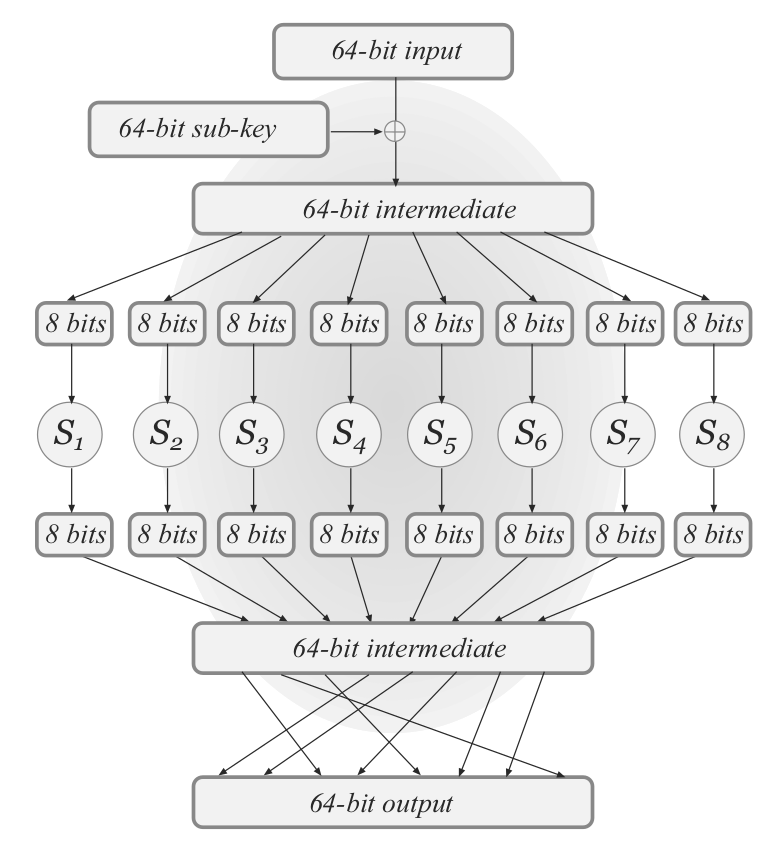
\includegraphics[width=0.5\linewidth]{2024-04-15-spn.png}
\end{center}

We can repeat this procedure for multiple rounds. For example, below is a 3-round SPN.

\begin{center}
    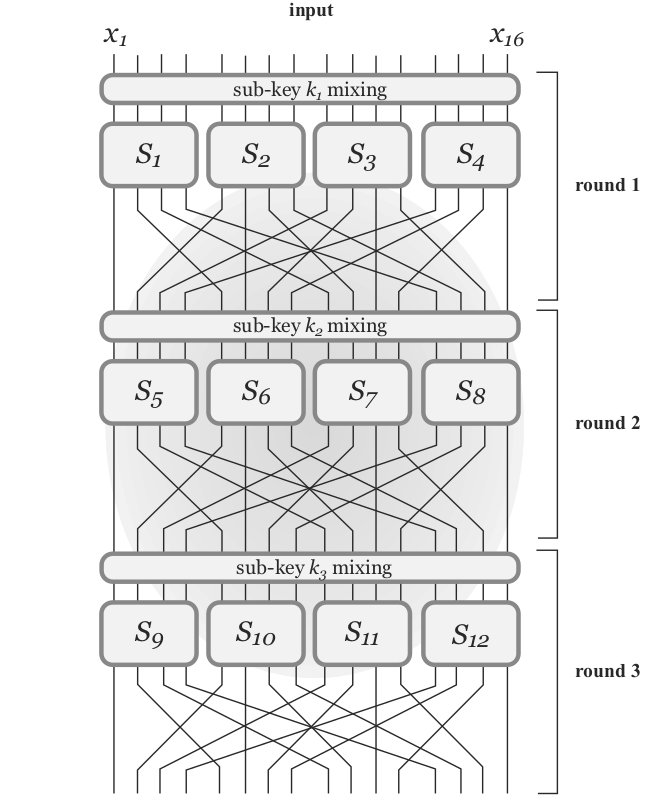
\includegraphics[width=0.5\linewidth]{2024-04-15-spn-mult.png}
\end{center}

Different sub-keys are used in each round. These sub-keys are derived from a \textit{master key} using a \textit{key schedule}, for example, by taking different subsets from the master key.

Given the master key, we can compute $F_{k}^{-1}(y)$. First, use the key schedule to find each sub-key, which we can use to XOR to get the inverse. Then, since each mixing permutation is public, we can compute its inverse for each round. Additionally, each S-box is public, so we can find its inverse too. Thus we have all the information we need to compute the inverse.

\subsection{Attacks on Reduced-Round SPN}

\textbf{1-round SPN without final key mixing.} The adversary can begin with the output $y$, then invert it starting from the end to the beginning. Since the permutations are public, the adversary can compute $x \oplus k$, and since they know the input $x$, they can figure out $k$. Thus we have a complete break. This shows that we need a final key mixing step.

\textbf{1-round SPN with final key mixing.} Assume the key and input is 16-bit. The adversary can try to attack by enumerate the possible values of $k_2$, then using the SPN derive $k_1$ for each $k_2$. This takes $O(2^{16})$ time and gives $2^{16}$ possible values for the master key.

\subsection{Feistel Network}

\begin{center}
    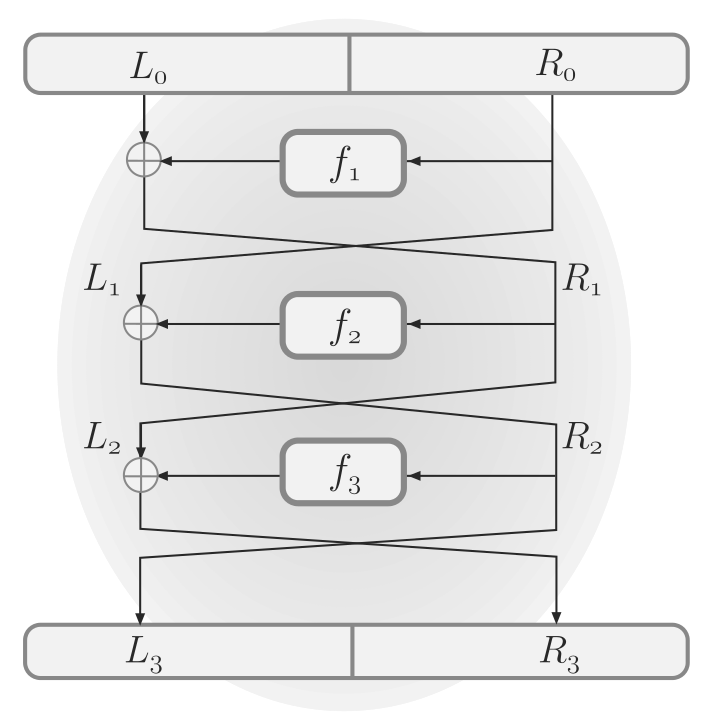
\includegraphics[width=0.5\linewidth]{2024-04-15-feistel-3round.png}
\end{center}

Let $x = L_0 || R_0$ be the input split into two halves, left and right. The $R_0$ is fed into a \textit{round function} $f_1$ and is XOR-ed with $L_0$ to get $R_1$. Then $L_1$ is defined to be $R_0$. This is repeated for several rounds (3 rounds in the figure above). Let $y= L_n || R_n$ be the output after $n$ rounds.

To compute the inverse $F_k^{-1}(y)$, start from the output e.g. $(L_3, R_3)$. We know $R_2 = L_3$, so we can compute $f_3(R_2)$. This satisfies $f_3(R_2) \oplus L_2 = R_3$, so we can find $L_2$. Thus we have found $(L_2, R_2)$, and we can continue until we get $x$.

There are attacks on reduced-round Feistel Networks that we will not cover in lecture, but you can think about it on your own.

\subsection{Data Encryption Standard (DES)}

Recall that the block length is $n=64$ and master key length is $\lambda = 56$ for DES. Use the Feistel network on our $64$-bit input $x$ so that $L_0, R_0$ each get $32$ bits. For the round functions, we use something called a \textit{DES mangler function}, which is essentially a SPN.

However, unlike an SPN, the S-boxes are not permutation, but rather they reduce the size from 6-bit to 4-bit. Additionally, the follow the following properties
\begin{enumerate}
    \item Maps $\{0, 1\}^6 \to \{0, 1\}^4$.
    \item ``4-to-1'': Exactly 4 inputs map to the same output.
    \item 1-bit change of input gives at least 2-bit change in the output.
\end{enumerate}

\begin{center}
    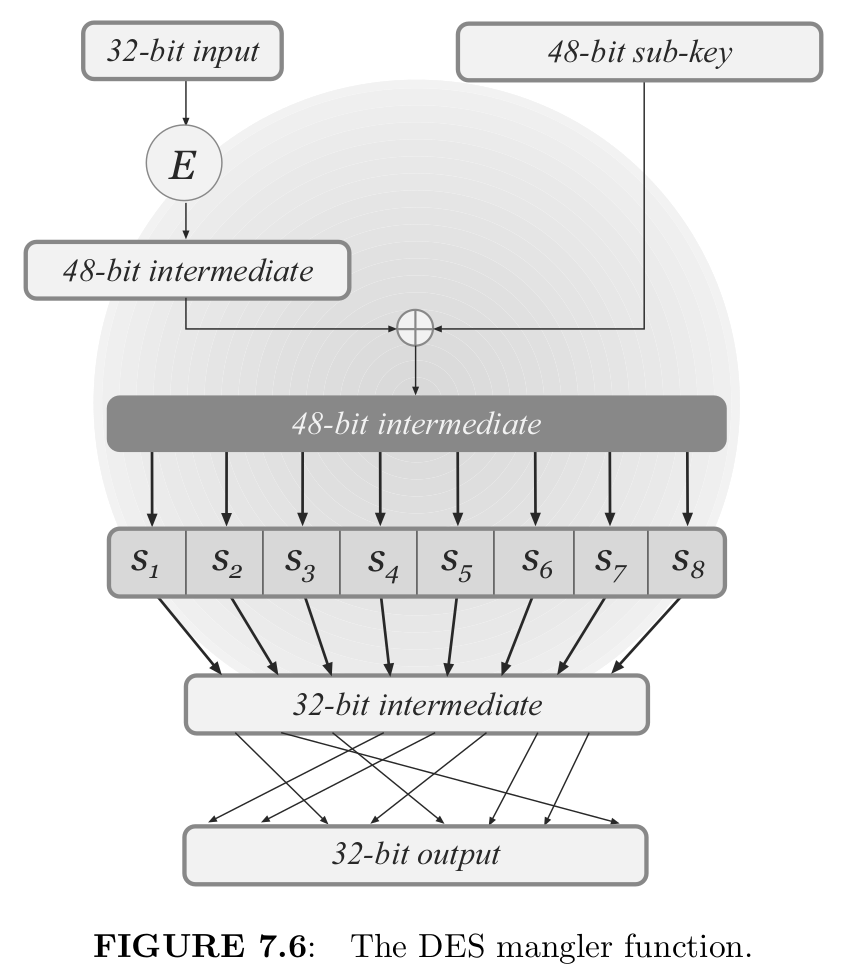
\includegraphics[width=0.5\linewidth]{2024-04-15-dsa-mangler.png}
\end{center}

$E$ is an expansion function. Given a 32-bit string AB where A and B are 16-bit, the output is a 42-bit string ABA.

For the key schedule, we have a master key with length 56 but need a 48-bit sub-key. To do so, split the master key into two halves of 28-bits each, then take a random subset of 24-bits from each half. Then concatenate these two subsets to form a 48-bit sub-key.

\begin{remark}
    DES does seem very complicated. This is intentional to do so so that attacks are hard.

    Multiple rounds of DES does not necessarily improve the security guarantees. Once DES is applied multiple times, we lose our security guarantee, and we need to do additional cryptanalysis, so it is unclear if it is secure. This is the reason NIST developed a new standard known as AES.
\end{remark}